\chapter{Disorder in Solids}
% \label{chap:2}



\section{Types of Disorder}

Disorder in solids refers to any deviation from perfect periodicity in the atomic arrangement. This can significantly alter electronic, optical, and transport properties, because the breaking of translational symmetry allows new scattering processes, modifies the density of states, and affects carrier dynamics \cite{Mahan2000,Kittel2005}.  

Disorder can be classified into several types:

\begin{itemize}
    \item \textbf{Substitutional disorder:} some lattice atoms are replaced by different species, modifying the local potential.
    \item \textbf{Interstitial disorder:} extra atoms occupy positions between the lattice sites.
    \item \textbf{Vacancies:} missing atoms that locally disrupt the potential.
    \item \textbf{Random displacements of atoms:} atoms are shifted randomly from their equilibrium lattice positions without changing the overall crystal structure.
    \item \textbf{Amorphous disorder:} no long-range order; the atomic positions are random beyond short-range correlations.
\end{itemize}

In this work, we focus on two cases in silicon:

1. \textbf{Random atomic displacements} within the crystal lattice (corresponding to weak disorder). This can be treated using standard scattering theory (Born approximation) and leads to finite lifetimes, spectral broadening, and band shifts.
2. \textbf{Amorphous silicon}, which is strongly disordered and exhibits Anderson-type localization. This requires non-perturbative treatment and modifies the transport properties and optical response dramatically \cite{Anderson1958,Economou2006,You2017}.

Disorder affects observable properties such as:

\begin{itemize}
    \item Band structure and density of states (DOS)
    \item Spectral broadening and self-energy corrections
    \item Optical absorption and high-harmonic generation
    \item Carrier transport and relaxation times
\end{itemize}








\section{Static Disorder and Scattering Theory}
\label{sec:RandomSi}

In crystalline silicon with small random atomic displacements, the electrons near the $\Gamma$ point of the conduction band can be described within the effective-mass approximation \cite{Kittel2005,YuCardona2010}. The dynamics are governed by the Hamiltonian
\begin{equation}
H = -\frac{\hbar^2}{2 m^\ast} \nabla^2 + \delta V(\mathbf{r}),
\end{equation}
where $m^\ast$ is the conduction-band effective mass and $\delta V(\mathbf{r})$ represents the disorder potential produced by stochastic atomic displacements.

\subsection{Disorder Potential and Scattering Framework}

The displacement of an atom from its equilibrium position modifies the local potential. In the regime of small atomic shifts, the perturbation can be modeled as a short-range scatterer. A widely used approximation in scattering theory \cite{Mahan2000,Economou2006} is to represent each displacement-induced perturbation by a delta-function potential,
\begin{equation}
\delta V(\mathbf{r}) = \sum_{n} V_0 \, \delta(\mathbf{r} - \mathbf{R}_n),
\end{equation}
where $V_0$ characterizes the strength of the displacement-induced potential.  
Such delta-like representations are routinely used in analytical disorder models \cite{Schirmacher2009,Paul1Ddisorder2017}.

The matrix element entering the Born approximation is \cite{Mahan2000}
\begin{equation}
|\langle \mathbf{k}' | \delta V | \mathbf{k} \rangle|^2 = \frac{V_0^2}{V^2},
\end{equation}
so scattering is isotropic and independent of the momenta.

\subsection{Effective-Mass Dispersion and Green's Function}

The conduction-band dispersion at the $\Gamma$ point is approximated as \cite{YuCardona2010}
\begin{equation}
E_{\mathbf{k}} = E_c + \frac{\hbar^2 k^2}{2 m^\ast},
\end{equation}
and the free retarded Green's function (see \cite{Economou2006}) is
\begin{equation}
G_0(E,\mathbf{k}) = \frac{1}{E - E_{\mathbf{k}} + i 0^+}.
\end{equation}

\subsection{Self-Energy in the Born Approximation}

In single-particle scattering theory, the disorder-averaged self-energy in the Born approximation \cite{Mahan2000,OminatoKoshino2013} is
\begin{equation}
\Sigma(E) = n_i V_0^2 
\int \frac{d^3 k}{(2\pi)^3}
\frac{1}{E - E_{\mathbf{k}} + i 0^+}.
\label{eq:SigmaBorn}
\end{equation}

Using the effective-mass DOS \cite{Kittel2005}
\begin{equation}
\rho_0(E) = 
\frac{1}{2\pi^2}
\left(\frac{2 m^\ast}{\hbar^2}\right)^{3/2}
\sqrt{E - E_c}
\;\Theta(E - E_c),
\end{equation}
Eq.~(\ref{eq:SigmaBorn}) yields \cite{Mahan2000}
\begin{equation}
\Im \Sigma(E) = -\pi n_i V_0^2 \rho_0(E),
\qquad
\Re \Sigma(E) = n_i V_0^2 
\, \mathcal{P}
\int dE'\, \frac{\rho_0(E')}{E - E'}.
\end{equation}

\subsection{Spectral Broadening}

The disorder-induced linewidth is therefore
\begin{equation}
\Gamma(E) = -2 \Im \Sigma(E)
           = 2\pi n_i V_0^2 \rho_0(E),
\end{equation}
an expression standard in scattering theory \cite{Mahan2000}.

Because $\rho_0(E) \propto \sqrt{E - E_c} \;\Theta(E - E_c)$, the width increases as
\begin{equation}
\Gamma(E) \propto \sqrt{E - E_c} \;\Theta(E - E_c).
\end{equation}

\subsection{Spectral Function}

The disorder-averaged Green's function becomes
\begin{equation}
G(E,\mathbf{k}) = 
\frac{1}{E - E_{\mathbf{k}} -\Sigma(E)} = 
\frac{1}{E - E_{\mathbf{k}} - \Re\Sigma(E) + i \Gamma(E)/2},
\end{equation}
and the spectral function is \cite{Mahan2000}
\begin{equation}
A(E,\mathbf{k}) = 
-\frac{1}{\pi}\Im G(E,\mathbf{k})
= \frac{1}{\pi}
\frac{\Gamma(E)/2}{
       \big(E - E_{\mathbf{k}} - \Re\Sigma(E)\big)^2
     + (\Gamma(E)/2)^2 }.
\end{equation}

\subsection{Scattering Rate}

The scattering rate follows directly:
\begin{equation}
\frac{1}{\tau(E)} = \frac{\Gamma(E)}{\hbar}
 = \frac{2\pi}{\hbar} n_i V_0^2 \rho_0(E),
\end{equation}
which is the standard Fermi golden rule for short-range impurities \cite{Mahan2000,Kittel2005}.

\subsection{Transport Time}

The transport time is given by \cite{Mahan2000}
\begin{equation}
\frac{1}{\tau_{\mathrm{tr}}(E)} =
\frac{2\pi}{\hbar} n_i V_0^2
\int \frac{d^3 k'}{(2\pi)^3}
(1 - \cos\theta_{\mathbf{k}\mathbf{k}'})
\delta(E_{\mathbf{k}} - E_{\mathbf{k}'}).
\end{equation}

For isotropic $\delta$-scatterers,
\begin{equation}
\tau_{\mathrm{tr}}(E) = \tau(E),
\end{equation}
as discussed in \cite{Mahan2000,Schirmacher2009}.

\subsection{Optical Absorption}

In linear response, the intraband absorption coefficient reads \cite{YuCardona2010}
\begin{equation}
\alpha(\omega) \propto
\int dE\,
A(E) A(E+\hbar\omega)
\big[ f(E) - f(E+\hbar\omega) \big].
\end{equation}

For Lorentzian broadening,
\begin{equation}
\alpha(\omega) \propto 
\frac{\Gamma(E)/2}{\omega^2 + (\Gamma(E)/2)^2},
\end{equation}
the standard result of broadened intraband transitions \cite{Mahan2000}.

\subsection{Density of States Modification}

The disorder-modified DOS is
\begin{equation}
\rho(E) =
\int \frac{d^3 k}{(2\pi)^3} A(E,\mathbf{k}),
\end{equation}
resulting in a broadened square-root onset at the band edge \cite{YuCardona2010}.

%%%%%%%%%%%%%%%%%%%%%%%%%%%%%%%%%%%%%%%%%%%%%%%%%%%%%%%%%%%%%%%
% ANALYTICAL BROADENED DOS
%%%%%%%%%%%%%%%%%%%%%%%%%%%%%%%%%%%%%%%%%%%%%%%%%%%%%%%%%%%%%%%

\subsection{Analytical Density of States for Parabolic Band with Scattering Broadening}
\label{subsec:DOS_broadened}

The clean DOS is \cite{YuCardona2010}
\begin{equation}
\label{eq:rho0_clean}
\rho_0(E)
=
\frac{1}{2\pi^2}
\left( \frac{2 m^\ast}{\hbar^2} \right)^{3/2}
\sqrt{E - E_c}
\;\Theta(E - E_c).
\end{equation}

To account for disorder-induced lifetime effects, we use the standard approximation from many-body scattering theory 
\cite{Mahan2000,Economou2006}

\[
\Sigma(E) = \Delta - i \Gamma/2 
\]
considering $\Delta$ and $\Gamma$ as constants, so that effectively
\[
E \rightarrow E - \Delta + i \Gamma/2.
\]

From general considerations, $\Delta$ is of the order of $\Gamma$ with an accuracy of logarithmic trimming. With second-order perturbation theory it can be shown that the sign of the delta must be negative so that the edge of the conduction band shifts downwards (while for the valence band, on the contrary, it shifts upwards).

If we make such a substitution in our previous formula for the case without defects we get the broadened DOS as the real part of the clean DOS evaluated at complex energy \cite{Mahan2000}:
\begin{equation}
\label{eq:rho_broad_def}
\rho(E) = 
\Re\!\left[
C \sqrt{(E - E_c - \Delta) + i\frac{\Gamma}{2}}
\right],
\end{equation}
with
\[
C =
\frac{1}{2\pi^2}
\left(\frac{2 m^\ast}{\hbar^2}\right)^{3/2}.
\]

A more rigorous derivation can be found in the \ref{sec:analytical_integral}.

Here we defined $E_c^* = E_c + \Delta$ Let $u = E - E_c^*$, $v = \Gamma/2$, and 
$R=\sqrt{u^2+v^2}$.  
Using the standard expression for complex square roots \cite{Economou2006},
\[
\sqrt{u + iv}
=
\sqrt{\frac{R + u}{2}}
+ i \sqrt{\frac{R - u}{2}},
\]
the broadened DOS becomes
\begin{equation}
\label{eq:rho_final}
\rho(E) =
C \sqrt{
\frac{
\sqrt{(E - E_c^*)^2 + (\Gamma/2)^2}
+ (E - E_c^*)
}{2}
}.
\end{equation}

This expression reduces to the clean DOS~(\ref{eq:rho0_clean}) when $\Gamma\rightarrow 0$, and produces a finite sub-gap tail characteristic of disorder broadening. Thus we can say that we have a broadening of the order of $\Gamma$. Real silicon with static defects (preserving the crystal structure) can have a band gap width reduction of about 0.1-0.2 eV. This gives a relaxation time of about 20-40 fs.


\begin{figure}[h!] % можно [t], [b], [p], [h]
    \centering
    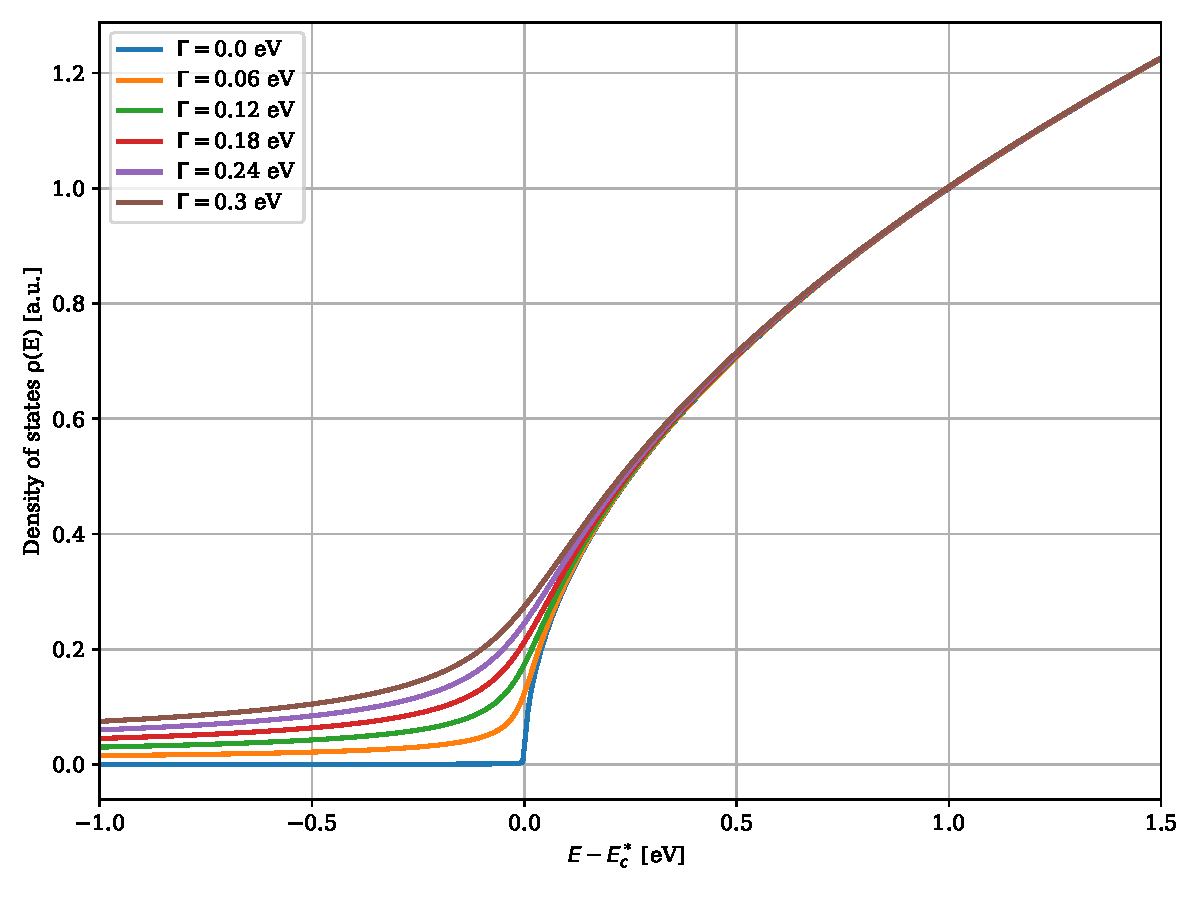
\includegraphics[width=0.7\linewidth]{figures/broadening.pdf} % путь к файлу
    \caption{Broadening according to \eqref{eq:rho_final}. For negative values of energy relative to the conduction band edge, we have the asymptotics $1/\sqrt{|E-E_c^*|}$}
    \label{fig:myimage}
\end{figure}






\subsection{Degeneracy Considerations for Scattering at the $\Gamma$ Point}

For the conduction band in silicon, the $\Gamma$ point corresponds to a 
non-degenerate conduction-band minimum (up to trivial spin degeneracy), as 
established in standard band-structure analyses \cite{Kittel2005,YuCardona2010}.  
Because of the full cubic symmetry of the diamond lattice, the effective-mass 
tensor at $\Gamma$ is isotropic, and the dispersion may be accurately 
approximated by a single parabolic band.  
Therefore, the standard single-band scattering formalism---including the 
Born approximation, scalar self-energy, Lorentzian spectral broadening, and 
the use of short-range disorder potentials---is directly applicable 
\cite{Mahan2000,Economou2006}.

In contrast, the valence band exhibits a strong degeneracy at the 
$\Gamma$ point: the heavy-hole (HH) and light-hole (LH) subbands are 
degenerate at $k=0$, forming the $J=3/2$ Luttinger multiplet 
\cite{Luttinger1956,Dresselhaus2008}.  
Because the valence-band states are multi-component spinors transforming 
under this representation, disorder does not act on a scalar wave function 
but on a matrix structure in the $\{HH, LH\}$ basis.  
Consequently, the scattering problem becomes intrinsically multiband: the 
self-energy, Green's function, and T-matrix are matrix-valued objects, and 
disorder generically mixes HH and LH components for $k\neq0$.  
A consistent treatment therefore requires the use of multiband $k\cdot p$ 
theory or the Luttinger-Kohn formalism \cite{YuCardona2010,Luttinger1956}.

Thus, while single-band scattering theory is fully appropriate for the 
conduction band at the $\Gamma$ point, the valence band requires a 
multiband scattering framework due to degeneracy and the anisotropic 
structure of the underlying $J=3/2$ manifold.






\section{Applicability of the Drude model}



In \cite{PhysRevB.79.115306} the authors show that the carrier transport depends strongly on microstructure:

\begin{itemize}
\item \textbf{Microcrystalline silicon (µc-Si:H):}
      carriers initially occupy extended states and produce a clear 
      Drude response. Over hundreds of femtoseconds they relax into 
      weakly and strongly localized states, yielding Debye and Dyre
      contributions.
\item \textbf{Amorphous silicon (a-Si:H):}
      carriers are trapped on ultrafast timescales (\(< 100\) fs), so
      no measurable Drude response appears; only Debye and Dyre
      conductivity is observed.
\end{itemize}

They use the model that describes the total conductivity as a sum of three physically distinct
channels:
\[
\sigma(\omega,t)
=
\sigma_{\mathrm{D}}(\omega,t)
+
\sigma_{\mathrm{R}}(\omega,t)
+
\sigma_{\mathrm{H}}(\omega,t).
\]


%--------------------------------------------------------------------
\subsection{Drude Conductivity (Delocalized Carriers)}

Delocalized carriers in extended states produce a Drude response:
\[
\sigma_{\mathrm{D}}(\omega,t)
=
\frac{ n_{\mathrm{free}}(t) e^2 \tau_{\mathrm{D}} }
     { m^\ast \left( 1 + i \, \omega \, \tau_{\mathrm{D}} \right) }.
\]
At low frequency,
\[
\lim_{\omega\to 0} \sigma_{\mathrm{D}}(\omega) = 
\frac{n_{\mathrm{free}} e^2\tau_{\mathrm{D}}}{m^\ast} > 0,
\]
indicating true DC conductivity and an inductive imaginary part
(\(\mathrm{Im}\,\sigma_{\mathrm{D}} < 0\)).


%--------------------------------------------------------------------
\subsection{Debye Relaxation (Weak Localization)}

Weakly localized carriers respond through dipolar relaxation. The
polarization obeys
\[
\dot{P} + \frac{P}{\tau_R} = \varepsilon_0 \Delta\varepsilon \, E,
\]
which yields the Debye conductivity:
\[
\sigma_{\mathrm{R}}(\omega,t)
=
\frac{i \omega \varepsilon_0 \Delta\varepsilon\, n_{\mathrm{rel}}(t)}
     {1 + i\omega \tau_R } .
\]
Separating real and imaginary parts:
\[
\sigma_{1,\mathrm{R}}(\omega,t)
=
\frac{ \omega^2 \varepsilon_0 \Delta\varepsilon\, n_{\mathrm{rel}}(t)\, \tau_R }
     { 1 + \omega^2 \tau_R^2 },
\qquad
\sigma_{2,\mathrm{R}}(\omega,t)
=
\frac{ \omega \varepsilon_0 \Delta\varepsilon\, n_{\mathrm{rel}}(t) }
     { 1 + \omega^2 \tau_R^2 } .
\]
Key properties:
\[
\lim_{\omega\to 0} \sigma_{1,\mathrm{R}} = 0,
\qquad
\mathrm{Im}[\sigma_{\mathrm{R}}] > 0.
\]
Thus Debye relaxation is \emph{purely capacitive} and carries no DC
conductivity, in sharp contrast to Drude.


%--------------------------------------------------------------------
\subsection{Dyre Hopping Conductivity (Strong Localization)}

Strongly localized carriers hop between spatially random localized
states. The Dyre model yields a dispersive hopping response:
\[
\sigma_{\mathrm{H}}(\omega,t)
=
n_{\mathrm{hop}}(t)\, e \mu_0
\;-\;
i\, n_{\mathrm{hop}}(t)\, e\,
\omega \tau_{\min} \mu_{\mathrm{H}}
\ln\!\bigl( 1 + \omega^2 \tau_{\min}^2 \bigr).
\]
\textcolor{red}{check}
This model produces the characteristic increase of
\(\sigma_1(\omega)\) with frequency at low \(\omega\), and a purely
capacitive imaginary response (\(\mathrm{Im}\,\sigma_{\mathrm{H}} > 0\)).


%--------------------------------------------------------------------
\subsection{Timescale Considerations}

On ultrashort delays,
\[
t \lesssim 100~\mathrm{fs},
\]
carriers in microcrystalline silicon remain in extended states. Hence
\[
\sigma(\omega, t \lesssim 100\ \mathrm{fs})
\;\approx\;
\sigma_{\mathrm{D}}(\omega,t),
\]
and the transient probe response is dominated by the Drude contribution.

In amorphous silicon, however, carriers are trapped on comparable or
shorter timescales, and the Drude term is absent even at the earliest
measurable delays. The response is therefore entirely due to Debye and
Dyre processes.

This is exactly what we can directly extract from our calculations and understand what type of conductivity we have.








% \newpage



% \section{Amorphous Silicon and Anderson Localization}

% Amorphous silicon lacks long-range crystalline order, leading to strong disorder that cannot be treated perturbatively. In this regime, electron dynamics are often described using Anderson-type Hamiltonians \cite{Anderson1958,Economou2006}:

% \begin{equation}
% \label{eq:H_anderson}
% H = \sum_i \epsilon_i c_i^\dagger c_i + \sum_{\langle i,j \rangle} t_{ij} c_i^\dagger c_j,
% \end{equation}
% where \(c_i^\dagger\) (\(c_i\)) creates (annihilates) an electron at site \(i\), \(t_{ij}\) are hopping elements, and \(\epsilon_i\) are on-site energies drawn from a random distribution with width \(W\).

% \subsection{Spectral Function and DOS (General Form)}

% The retarded Green's function is defined as
% \begin{equation}
% \label{eq:G_ret}
% G_{ij}(E) = \langle i | \frac{1}{E - H + i0^+} | j \rangle.
% \end{equation}

% The spectral function at site \(i\) is
% \begin{equation}
% \label{eq:spectral_anderson}
% A_i(E) = -\frac{1}{\pi} \Im G_{ii}(E),
% \end{equation}
% and the total density of states (DOS) is
% \begin{equation}
% \label{eq:DOS_anderson}
% \rho(E) = \frac{1}{N} \sum_i A_i(E).
% \end{equation}

% \subsection{Optical Absorption (General Form)}

% For a tight-binding model, the optical absorption is
% \begin{equation}
% \label{eq:absorption_anderson}
% \alpha(\omega) \propto \sum_{i,j} |\langle i | \hat{\mathbf{e}} \cdot \mathbf{r} | j \rangle|^2 \int dE \, A_i(E) A_j(E+\hbar\omega) [f(E) - f(E+\hbar\omega)].
% \end{equation}

% \subsection{Transport Time and Localization}

% The transport (or diffusion) time in the presence of strong disorder can be estimated via the Kubo-Greenwood formula:
% \begin{equation}
% \label{eq:transport_anderson}
% \frac{1}{\tau_{\rm tr}} = \frac{2\pi}{\hbar} \sum_{i,j} |\langle i | \hat{v} | j \rangle|^2 A_i(E_F) A_j(E_F),
% \end{equation}
% where \(\hat{v}\) is the velocity operator and \(E_F\) is the Fermi energy.  

% Strong disorder leads to \textbf{Anderson localization}, characterized by exponentially decaying wavefunctions:
% \begin{equation}
% \psi_n(r) \sim e^{-r/\xi},
% \end{equation}
% where \(\xi\) is the localization length. For localized states, transport is suppressed (\(\tau_{\rm tr} \rightarrow \infty\) in the thermodynamic limit), and the DOS may develop \textbf{Urbach tails} \cite{Abkowitz1984}.

% \subsection{Analytical Examples}

% \textbf{1. 1D Anderson Model with Uniform Disorder} (\(\epsilon_i \in [-W/2, W/2]\)):

% \[
% \rho(E) \approx \frac{1}{\pi \sqrt{4t^2 - E^2}}, \quad |E| < 2t,
% \]

% broadened by disorder via convolution with the distribution of \(\epsilon_i\).  

% \textbf{2. Delta-function Impurity Model in 3D:} Consider a cubic lattice with hopping \(t\) and on-site delta-function potential \(V_0\) at random sites with concentration \(c\). Then the self-energy in the coherent potential approximation (CPA) is
% \[
% \Sigma(E) = \frac{c V_0}{1 - (V_0 - \Sigma(E)) G_0(E)},
% \]
% where \(G_0(E)\) is the Green’s function of the pure lattice. The spectral function is
% \[
% A(E) = -\frac{1}{\pi} \Im \frac{1}{E - \Sigma(E) - H_0}.
% \]
% This gives analytic estimates of spectral broadening and band edge shifts \cite{Economou2006}.

% \textbf{3. Transport Time for Weak Hopping Limit:} For strong disorder but small \(t\), transport can be estimated as
% \[
% \frac{1}{\tau_{\rm tr}} \sim \frac{t^2}{\hbar W},
% \]
% showing suppression of conductivity with increasing disorder strength.

% \medskip

% \textbf{References:} Anderson \cite{Anderson1958}, Economou \cite{Economou2006}, Abkowitz \cite{Abkowitz1984}, Ominato \& Koshino \cite{OminatoKoshino2013} (analytical SCBA examples), Yu \& Cardona \cite{YuCardona2010} (optical absorption).







% \section{Summary}

% This work investigated the effects of disorder on the electronic and optical properties of silicon, focusing on two regimes: random atomic displacements in crystalline silicon and amorphous silicon exhibiting Anderson localization.

% For crystalline silicon with small atomic displacements, we analyzed how disorder affects the self-energy, spectral function, density of states, optical absorption, and transport time. In simple analytical models, such as delta-function atomic potentials, disorder leads to broadening of spectral lines, shifts of energy levels, and finite transport times \cite{OminatoKoshino2013,Schirmacher2009,Paul1Ddisorder2017,YuCardona2010}.

% In amorphous silicon, strong disorder results in localized electronic states and suppression of transport. Analytical and numerical models based on Anderson-type Hamiltonians describe the density of states, spectral function, optical absorption, and transport in this regime \cite{Anderson1958,Economou2006,Abkowitz1984}. 

% Overall, the study provides a unified framework to understand how disorder modifies electronic and optical responses in silicon, with direct relevance for attosecond spectroscopy experiments.




\section{Dataset of Amorphous Silicon Structures}

In this work we will use dataset of amorphous structures from~\cite{rosset2024signaturesparacrystallinityamorphoussilicon}.

To characterize atomic environments, Rosset \emph{et al.} employ the Smooth
Overlap of Atomic Positions (SOAP) descriptor.


For each atom $i$, we define a neighbor density
\begin{equation}
  \rho_i(\mathbf{r})
  =
  \sum_{j}
  \exp\!\left(
    -\frac{|\mathbf{r}-\mathbf{r}_{ij}|^2}{2\sigma^2}
  \right)
  f_c(|\mathbf{r}_{ij}|),
  \label{eq:rho_i}
\end{equation}
where the sum runs over neighbors $j$ within the cutoff radius $r_c$.
Here $\sigma$ is the Gaussian smearing width and $f_c(r)$ is a smooth cutoff
function.


Then we expand the density~\eqref{eq:rho_i} in orthonormal radial functions
$g_n(r)$ and spherical harmonics $Y_{\ell m}$:
\begin{equation}
  \rho_i(\mathbf{r})
  =
  \sum_{n\ell m}
  c_{n\ell m}^{(i)}\,
  g_n(r)\,
  Y_{\ell m}(\hat{\mathbf{r}}),
  \label{eq:rho_expansion}
\end{equation}
where $c_{n\ell m}^{(i)}$ are expansion coefficients.
Rotational invariance is achieved by constructing the SOAP power spectrum
\begin{equation}
  p^{(i)}_{nn'\ell}
  =
  \sum_{m}
  c_{n\ell m}^{(i)\,*}
  c_{n'\ell m}^{(i)},
  \label{eq:SOAP_powerspec}
\end{equation}
which serves as the rotationally invariant descriptor vector
$\mathbf{p}^{(i)}$.

Similarity between environments $i$ and $k$ is quantified using the SOAP kernel
\begin{equation}
  k_\mathrm{SOAP}(i,k)
  =
  \left(
    \frac{
      \mathbf{p}^{(i)} \cdot \mathbf{p}^{(k)}
    }{
      \|\mathbf{p}^{(i)}\|\,
      \|\mathbf{p}^{(k)}\|
    }
  \right)^{\zeta},
  \label{eq:SOAP_kernel}
\end{equation}
where $\zeta\ge 1$ controls the sharpness of the similarity measure.
By construction,
\[
0 \le k_\mathrm{SOAP}(i,k) \le 1,
\]
with $k_\mathrm{SOAP}=1$ only for identical local structures (up to rotation).
Rosset \emph{et al.} use $k_\mathrm{SOAP}(i,\mathrm{diamond})$ to quantify how
closely a given local environment resembles crystalline diamond-structure
silicon, enabling continuous discrimination between amorphous, paracrystalline,
and crystalline domains.






% \section{Random Displacements From Equilibrium Positions}
% \lipsum[1]

% \section{Amorphous Disorder}
% \lipsum[1]

% \subsection{SOAP Function}

% \lipsum[1]

% \section{Energy Band Diagram}
% \lipsum[1]

% \subsection{Absorption Spectrum}
% \lipsum[1]